\chapter{Listning Test}\label{app:journal_ListningTest}

This test was performed to investigated whether it is more pleasant to listen to a multi-band compressor or a single-band compressor. In order to give a broad selection of answers 10 people were randomly chosen to listen to four different types of music without knowing what type of effect block they were subjected to.


\section{Setup}



\begin{itemize}\addtolength{\itemsep}{-.35\baselineskip} 
\item A Person will be placed approximately 2-3 meters from the loudspeaker
\item The speaker will be driven by a Crown Studio Reference I amplifier.
\item The person will be placed directly in front of a single speaker
\item The power of the speaker will be adjusted to output a \gls{SPL} of approximately 80-83 dB(A)
\item The playback unit will be a computer
\item The playback unit will be connected via. 3.5 mm minijack cable to the amplifier
\end{itemize}
\vspace{-5mm}
Furthermore the speaker will be placed in a listing room to give as natural a response as possible. The room conforms with the ITU-R BS775-1 standard for multichannel systems.

The clips used are originating from following songs:
\vspace{-5mm}
\begin{enumerate}\addtolength{\itemsep}{-.35\baselineskip} 
\item Shots \& Squats by Vigiland
\item Sultans Of Swings by Dire Straits
\item Stormy Weather by Teitur
\item Hearth Of Courage by Two Steps From Hell
\end{enumerate}
Test clips can be found on \path{CD://ListningTestFiles/RefX.wav} where X corresponds to the index number of the song.
The Songs are mastered with the following effectblocks via Logic Pro:

\noindent\begin{minipage}[t]{0.5\linewidth}
    \textbf{Singleband:}
    \begin{itemize}\addtolength{\itemsep}{-.35\baselineskip} 
    \item 1 band in entire frequency spectrum
    \item 12 dB attenuation at 0 dBFS
    \item Attack time of 0.5 ms and release time of 1 ms
    \end{itemize}
    \end{minipage}%
    \begin{minipage}[t]{0.5\linewidth}
    \textbf{Multiband:}
    \begin{itemize}\addtolength{\itemsep}{-.35\baselineskip} 
    \item 1 band from 0 to 100 Hz
    \item 1 band from 100 to 300 Hz
    \item 1 band from 300 to 1000 Hz
    \item 1 Limiter in entire frequency spectrum
    \item Attack time of 0.5 ms and release time of 1 ms
    \end{itemize}
\end{minipage}\par\bigskip
Test clips can be found on \path{CD://ListningTestFiles/} as \path{MultiX.wav} and \path{SingleX.wav} respectively where X corresponds to the index number of the song.



\subsection*{Test Setup}
The setup inside the rooms is done as displayed on \autoref{figure:SpeakertestSetupListning}. The Person is placed in a chair in front of one speaker.
\begin{figure}[H]
\centering
\tikzsetnextfilename{TestSetupListning}
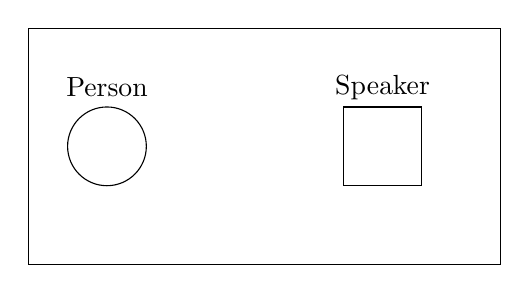
\begin{tikzpicture}
\draw  (-3,2) rectangle (3,-1);
\draw  (2,1) rectangle (1,0);
\draw  (-2,0.5) ellipse (0.5 and 0.5);
\node at (-2,1.25) {Person};
\node at (1.5,1.25) {Speaker};
\end{tikzpicture}
\caption{Test setup}
\label{figure:SpeakertestSetupListning}
\end{figure}

\subsection*{Equipment used and AAU-no.}

\begin{table}[H]
\centering
\ra{1.3}
\begin{tabular}{S[table-format=1]ccc} \toprule
    {Item} & {Description} & {AAU-no} \\ \bottomrule 
    1      &  Monacor Sound Level Meter - SM-4      & 08132   \\
    4      &  Crown Studio Reference I Amplifier    & 52614   \\
    6      &  B \& K Microphone calibrator 4231     & 78301   \\
    8      &  Computer                              & NaN     \\  
    8      &  Passive Dali Zensor 5 AX              & NaN     \\ \bottomrule 
\end{tabular}
\caption{Table over equipment used in test}
\label{tab:UsedEquipmentListning}
\end{table}



\section{Procedure}\label{sec:SpeakerTestProcedure3}

The producer for this experiment is described as follows:
\vspace*{-5mm}
\begin{enumerate}\addtolength{\itemsep}{-.35\baselineskip} 
\item Adjust volume of \gls{SPL} on all songs to approximately 80-83 dB.
\item Place test person in chair and explain procedure to him
\item Play \path{RefX.wav}
\item Play \path{MultiX.wav} and ask test subject to choose the most favourable clip.
\item Play \path{SingleX.wav} and ask test subject to choose the most favourable clip.
\item Repeat step 3 through 4 with the X on the file incremented.
\end{enumerate}

\section{Data Extraction}
The answers given by the test subjects are located
The recordings can be found on:\\
\scalebox{0.7}{
\path{CD://ListningTestFiles/Lyttetest.excel}}\\
All of the data is inserted in tables where an x is placed on the outcome. The tables are shown in raw format in section \ref{sec:rawdata_listning}.



\section{Raw data}\label{sec:rawdata_listning}
The following sections shows tables where the discrete value of each trail is noted. A is multiband and B is singleband. The X marks the most favourable. 
\begin{figure}[H]
\centering
\begin{subfigure}[t]{0.20\textwidth}
\begin{table}[H]
\centering
\begin{tabular}{ccccc}
n        & A       & B       & A       & B      \\ \bottomrule 
1        & X       &         & X       &        \\
2        & X       &         & X       &        \\
3        & X       &         & X       &        \\
4        & X       &         &         & X      \\
5        & X       &         & X       &        \\ \hline
6        & X       &         &         & X      \\
7        & X       &         & X       &        \\
8        & X       &         & X       &        \\
9        & X       &         & X       &        \\
10       & X       &         & X       &        \\ \bottomrule 
\end{tabular}
\caption{Shots and Squats - Vigiland}
\label{tab:shotsandsquats}
\end{table}
\end{subfigure}
\hfill
\begin{subfigure}[t]{0.20\textwidth}
\begin{table}[H]
\centering
\begin{tabular}{ccccc}
n         & A        & B        & A       & B       \\ \bottomrule 
1         &          & X        & X       &         \\
2         & X        &          & X       &         \\
3         & X        &          & X       &         \\
4         & X        &          &         & X       \\
5         & X        &          & X       &         \\ \hline
6         &          & X        & X       &         \\
7         & X        &          & X       &         \\
8         & X        &          & X       &         \\
9         &          & X        &         & X       \\
10        & X        &          & X       &         \\ \bottomrule 
\end{tabular}
\caption{Sultans of swing - Dire Straits}
\label{tab:Sultansofswing}
\end{table}
\end{subfigure}
\hfill
\begin{subfigure}[t]{0.20\textwidth}
\begin{table}[H]
\centering
\begin{tabular}{ccccc}
n       & A      & B      & A      & B      \\ \bottomrule
1       & X      &        & X      &        \\
2       & X      &        & X      &        \\
3       & X      &        & X      &        \\
4       &        & X      &        & X      \\ 
5       & X      &        & X      &        \\ \hline
6       & X      &        & X      &        \\
7       & X      &        & X      &        \\
8       & X      &        & X      &        \\
9       & ?      & ?      & X      &        \\
10      & X      &        & X      &        \\ \bottomrule
\end{tabular}
\caption{Stormy Weather - Teitur}
\label{tab:stormyweather}
\end{table}
\end{subfigure}
\hfill
\begin{subfigure}[t]{0.20\textwidth}
\begin{table}[H]
\centering
\begin{tabular}{ccccc}
n          & A         & B         & A         & B        \\ \bottomrule
1          & X         &           & X         &          \\
2          & X         &           & X         &          \\
3          & X         &           & X         &          \\
4          & X         &           & X         &          \\ 
5          & X         &           & X         &          \\ \hline
6          & X         &           & X         &          \\
7          & X         &           & X         &          \\
8          & X         &           & X         &          \\
9          & X         &           & X         &          \\
10         & X         &           & X         &          \\ \bottomrule
\end{tabular}
\caption{Hearth of Courage - 2 Steps From Hell}
\label{tab:HearthofCourage}
\end{table}
\end{subfigure}

\caption{Tables showing what the test subjects asked. A symbols multi-band and B symbols single-band}
\label{tab:combinedanswers}
\end{figure}  

\vspace*{-5mm}
\section{Analysis}
The Raw data is first visualized in a pie chart, which creates a overview of how the answers of the test were placed. In \autoref{fig:piechartsongs} it shows this overview.
\begin{figure}[H]
\centering
\resizebox{0.5\textwidth}{!}{
\tikzsetnextfilename{Piechartsongs}
\begin{tikzpicture}
[
    pie chart,
    slice type={comet}{blu},
    slice type={legno}{rosso},
    slice type={coltello}{giallo},
    slice type={sedia}{viola},
    slice type={caffe}{verde},
    pie values/.style={font={\small}},
    scale=2
]
%    \pie{2008}{73/comet,13/legno,7/sedia,7/coltello}
%    \pie[xshift=2.2cm,values of coltello/.style={pos=1.1}]%
%        {2009}{52/comet,23/legno,17/sedia,3/coltello,5/caffe}
    \pie[values of caffe/.style={pos=1.1}]%
       {}{87.5/comet,10/legno,2.5/caffe}
%    \pie{2008}{87.5/comet,2.5/legno,10/sedia}
    \legend[shift={(1.5cm,0.5cm)}]{{Multiband}/comet, {Uncertain}/caffe, {Singleband}/legno}
%    \legend[shift={(3cm,-1cm)}]{{Chair (Manzano)}/sedia, {Coffee (Trieste)}/caffe}
\end{tikzpicture}}
\caption{Overall comparison of the answers}
\label{fig:piechartsongs}
\end{figure}

The raw data is further visualized in a bar chart showed in \autoref{fig:Barchartsongs} showing more a more in-depth visualization acording to each song. The bars are plotted showing the singleband and multiband compared directly to each other.
\begin{figure}[H]
\centering
\tikzsetnextfilename{Barchartsongs}
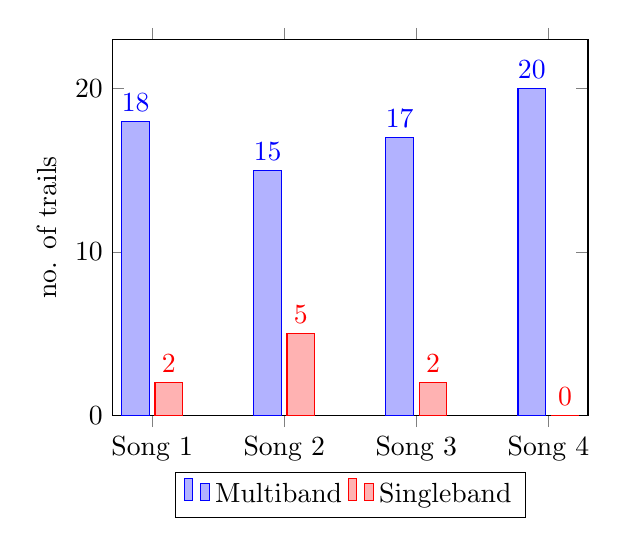
\begin{tikzpicture}
\begin{axis}[
	width=3.0in,
	height=2.5in,
    ybar,
%    enlargelimits=0.15,
    legend style={at={(0.5,-0.15)},
      anchor=north,legend columns=-1},
    ylabel={no. of trails},
    symbolic x coords={Song 1,Song 2,Song 3,Song 4},
    xtick=data,
    ymin=0,
    ymax=23,
    nodes near coords,
    nodes near coords align={vertical},
    ]
\addplot coordinates {(Song 1,18) (Song 2,15) (Song 3,17) (Song 4,20)};
\addplot coordinates {(Song 1,2)  (Song 2,5)  (Song 3,2) (Song 4,0)};
\legend{Multiband,Singleband}
\end{axis}
\end{tikzpicture}
\caption{Comparison of the different test}
\label{fig:Barchartsongs}
\end{figure}

\autoref{fig:piechartsongs} shows a strong tendency to the sound of a multiband compressor. Songs with a high using a high dynamic range shows a pattern of beeing more even more favourable with the mulitband compressor. This correlates to the fact that the singleband are to aggresive when attenuating. The sound becomes to distorted. This is especially the result of song 4. However, from \autoref{fig:Barchartsongs} the test result also shows that it becomes less important when more the clip contains more instruments in play at the same time. It shows that song 2 was slightly less attractive with the multiband. 


\section{Error sources}

There are two sources of error which could change the outcome of the result. The first error source is from the effect blocks used. They are not identical with the system developed and might be different in perception. The most dominant error source is the amount of people used in the test. There are only 10 people used in the experiment which might not be a sufficient enough sample.

\section{Conclusion}

The test showed a clear tendency of the multiband being more favourable when subjected to songs in the genres, dance, acoustics, pop/rock and instrumental. It showed that the singleband compressor had to much attenuation which made the music to distorted hence not favourable. The multiband compressor had better chance of only attenuating the problem frequencies.



